\section{Low Power Wide Area network}
\label{sec:overview-lpwa}
The term Low Power Wide Area network (LPWA) refers to a network relying on low power and wide area connectivity technology that simultaneously supports low batter energy consumption and wide coverage area. The LPWA network is dedicated to serve battery-powered applications characterized by low throughput, delay-tolerant and being event-driven such as water-meter monitoring. Unlike the other technologies that are adapted for IoT, LPWA networks are purposely designed from scratch to meet wide-area IoT application. 

LPWA technologies are typically narrow-band (with some exceptions) and operate in the ISM license-exempt spectrum bands. Faced with a potential huge market, lots of players propose their solutions. Some typical and already deployed proprietary technologies of LPWA network are LoRaWAN, SIGFOX, Weightless, OnRamp, etc. A comprehensive comparison about these existing LPWA solutions is shown in Tab.~\ref{tab:lpwan-comp}.
\begin{table}[!t]
	\centering
	\caption{The comparison among LPWAN solutions (All solutions are on ISM band, extracted from \cite{eejournal:lpwan})}
	\label{tab:lpwan-comp}
	\resizebox{\textwidth}{!}{%
		\begin{tabular}{@{}lllllclll@{}}
			\toprule
			& LoRaWAN                                                                           & NWave                                                               & OnRamp                                                                       & SIGFOX                                                       & \multicolumn{1}{l}{Telensa}                                                    & Weightless-N      & Weightless-P                                                                                        & Amber Wireless                                                      \\ \midrule
			\begin{tabular}[c]{@{}l@{}}Range\\ \\ (km)\\ (Caveat)\end{tabular}   & \begin{tabular}[c]{@{}l@{}}15-45 flat;\\ 15-22 suburban;\\ 3-8 urban\end{tabular} & 10                                                                  & \begin{tabular}[c]{@{}l@{}}4 \\ (but claims 25X\\  competition)\end{tabular} & \begin{tabular}[c]{@{}l@{}}50 rural;\\ 10 urban\end{tabular} & up to 8                                                                        & 5+                & 2+ urban                                                                                            & up to 20                                                            \\ \midrule
			\begin{tabular}[c]{@{}l@{}}Band\\ (MHz)\end{tabular}                 & \begin{tabular}[c]{@{}l@{}}spread; \\ varies by region\end{tabular}               & sub-GHz                                                             & 2.4 GHz                                                                      & 868;902                                                      & \begin{tabular}[c]{@{}c@{}}868/915\\ 470 (China)\end{tabular}                  & sub-GHz           & sub-GHz                                                                                             & 434, 868, 2.4GHz                                                    \\ \midrule
			\begin{tabular}[c]{@{}l@{}}Symmetric\\ up/down\end{tabular}          & \begin{tabular}[c]{@{}l@{}}depends on mode.\\ Can be\end{tabular}                 & no                                                                  & no(4:1)                                                                      & no                                                           & yes                                                                            & uplink only       & not yet determined                                                                                  &                                                                     \\ \midrule
			Data rate                                                            & \begin{tabular}[c]{@{}l@{}}0.3-50 kbps\\ (adaptive)\end{tabular}                  & 100 bps                                                             & 8 bps - 8 kpbs                                                               & 100 bps                                                      & low                                                                            & 30-100 kbps       & up to 100 kpbs                                                                                      & up to 500 kbps                                                      \\ \midrule
			\begin{tabular}[c]{@{}l@{}}Max nodes\\ (Caveat)\end{tabular}         & \begin{tabular}[c]{@{}l@{}}depends;\\ millions/hub\end{tabular}                   & million/base                                                        & "10s of 1000s"                                                               & millions/hub                                                & \begin{tabular}[c]{@{}c@{}}150,000/server\\ (moving to\\ 500,000)\end{tabular} &                   & \begin{tabular}[c]{@{}l@{}}32767 NWs,\\ 65535 hubs each, \\ 16 M edge device \\ per NW\end{tabular} & \begin{tabular}[c]{@{}l@{}}255 network \\ of 255 nodes\end{tabular} \\ \midrule
			\begin{tabular}[c]{@{}l@{}}Operational\\ model\end{tabular}          & \begin{tabular}[c]{@{}l@{}}public or private \\ (expect 80\% public)\end{tabular} & public or private                                                   & public or private                                                            & public                                                       & public                                                                         & public or private & public or private                                                                                   &                                                                     \\ \midrule
			\begin{tabular}[c]{@{}l@{}}Standard\\ status\\ (if any)\end{tabular} & \begin{tabular}[c]{@{}l@{}}LoRa: proprietary\\ LoRaWAN: yes\end{tabular}          & Weightless-N                                                        & no                                                                           & no                                                           & \begin{tabular}[c]{@{}c@{}}no\\ (perhaps in future)\end{tabular}               & yes               & in process                                                                                          &                                                                     \\ \bottomrule
		\end{tabular}
	}
\end{table}
LoRa alliance has issued their first vision of LoRaWAN specification \cite{lora/specification} in January 2015, which is regarded as a major step towards international standardization in field of LPWA networks. Thus, LoRaWAN (LoRa Wide Area Network) technology is taken as a concrete example to give a general view about LPWA networks. The network architecture is illustrated in Fig.~\ref{fig:lora-net-arch}, which is a star-of-stars topology. A LoRaWAN network consists of the following components \cite{lora/specification}:
\begin{figure}[!t]
	\centering
	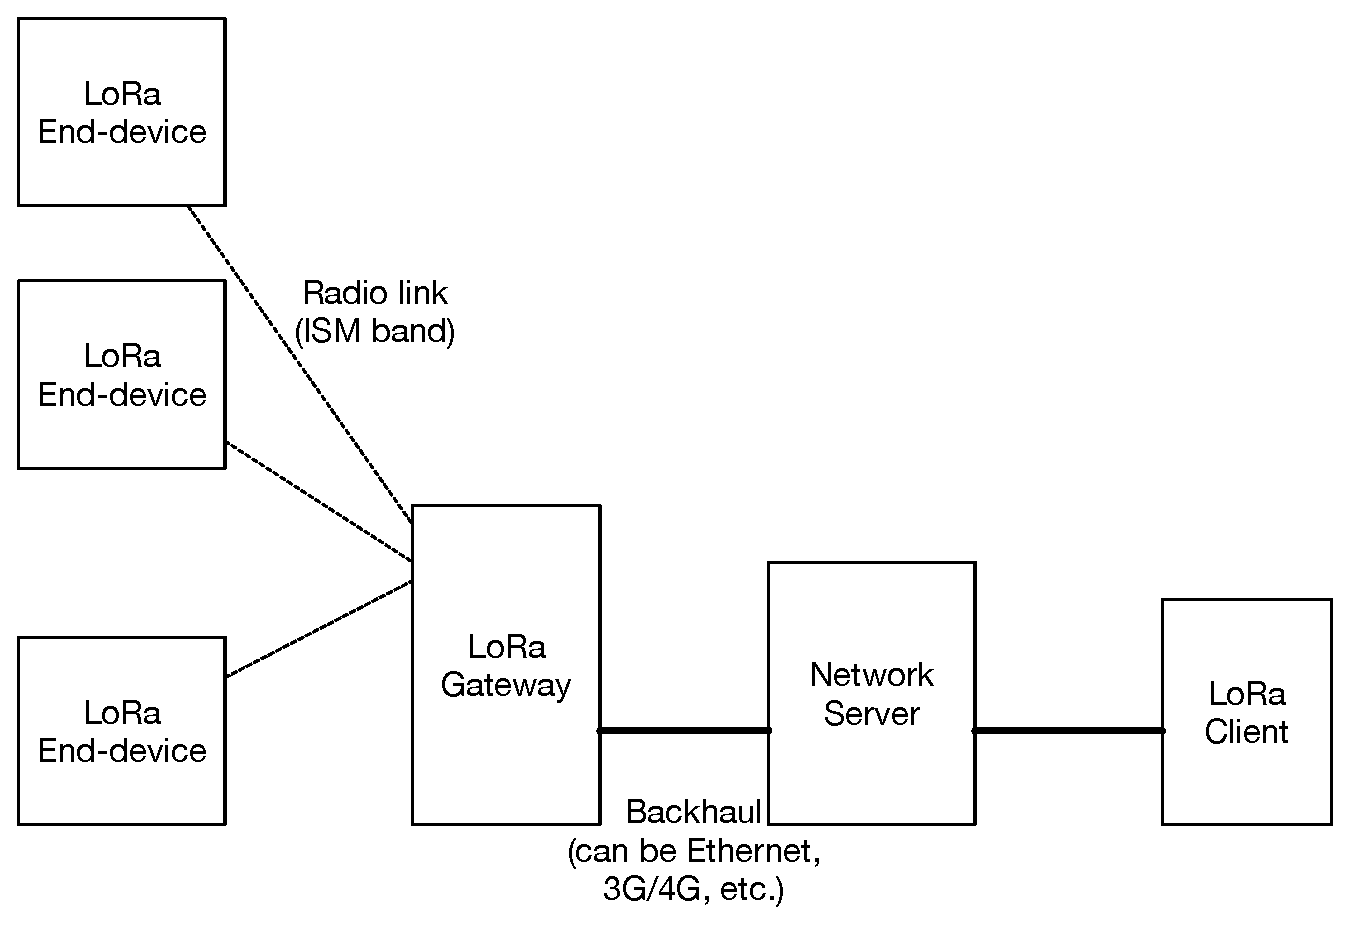
\includegraphics[width=0.8\linewidth]{Chapter2/Figures/LoRa-net-arch.eps}
	\caption{LoRaWAN network architecture. (based on \cite{lora/specification})}
	\label{fig:lora-net-arch}
\end{figure}
\begin{itemize}[leftmargin=*]
	%	http://www.radio-electronics.com/info/wireless/lora/lorawan-network-architecture.php
	\item End-device: the end-device is the element in a LoRaWAN network, which is responsible for collecting and uploading information to remote network server. LoRa supported functionalities can be classified to three classes: Class A (Bi-directional end-devices), Class B (Bi-directional end-devices with scheduled receive slots) and Class C (Bi-directional end-devices with maximal receive slots). All LoRaWAN end-devices at least support Class A. According to applications, end-devices can optionally support Class B and Class C.
	\item LoRa air interface: The LoRa air interface provides the connectivity between LoRa end-devices and gateway. It is on ISM (Industrial Scientific Medical) band and based on LoRa modulation, which is a proprietary modulation scheme. The LoRa data rate ranges from $0.3$ kbps to $50$ kbps. The selection of data rate is a trade-off between
	communication range and message duration, and communications with different data rates do
	not interfere with each other. 
	\item LoRa gateway: the LoRa gateway receives the communications from the LoRa end-devices and then transfers them to network server via the backhaul system. Note that LoRa gateways may be co-located with a cellular base station. In this way they are able to use spare capacity on the backhaul network.
	\item Network server:  the LoRa network server manages the network. The network server acts to eliminate duplicate packets, schedules acknowledgment, and adapts data rates (Adaptive Data Rate scheme). The communication between LoRa gateway and network server is IP-based, and the underlying carrier networks can be wired or wireless,  Ethernet or 3GPP cellular, public or private networks.
\end{itemize}

In order to answer the huge expected demand of cellular M2M coverage, the standardization organizations embarked on a process of standardizing narrow-band technology for use in mobile spectrum. Two possible tracks are addressed by the 3GPP. The first track is the evolution of LTE 3GPP cellular system with the objective of reducing the occupied bandwidth but still reusing the basic LTE principles. The second track is to propose a clean slate solution, which features narrow-band (NB) technologies and leverage the existing cellular infrastructure. One major difference between these two tracks relies in that whether it should redesign the radio interface and multiple access control mechanism for cellular M2M networks. 

As an effort in the first track, the 3GPP developed LTE-M specification in Rel-12 \cite{Nokia15} with introduction of a new low complexity device category (Cat-0). The device complexity of Cat-0 is $50$\% of the previously defined Cat-1, which is the basic LTE terminal defined in the first LTE Release (Rel-8). Nowadays, 3GPP is considering to further optimize LTE-M in Rel-13: 1) bandwidth of $1.4$ MHz and less complexity \cite{Nokia15}; 2) a narrow-band evolution of LTE-M with bandwidth $200$ kHz \cite{ratasuk2014narrowband}. 

For the clean slate solutions, the main idea is to sacrifice the data rate in order to gain energy efficiency and coverage extension. They are supposed to satisfy the following requirements: deployment in a small bandwidth (e.g. $200$ kHZ), ultra low-cost terminal (less than $5$ dollars), ultra-long battery life and coverage extension of $20$ dB with existing cellular technologies. The typical solutions include Narrow Band M2M (NB M2M), Narrow Band OFDMA, Cooperative Ultra Narrow Band (C-UNB) \cite{3GPP/cellularIoT}. The deployment options include re-farming GSM spectrum, LTE band guard and leftover fragments of spectrum during re-farming of 2G/3G to 4G. 

When these standards will be available, the cellular M2M connectivity solutions may be more competitive, since they not only fulfill the requirements of extended coverage and long battery life, but also have the advantage of being able to operate in currently existing cellular network, thus requiring no additional deployment of antennas, radio, or other hardware. On the contrary, the proprietary (at least for the time-being) technologies such as Sigfox, On-Ramp and LoRaWAN require a dedicated network and maintenance team to deploy and maintain their services, which increases operational complexity for the operator. However, their M2M solution is currently available for the operators and start to occupy some share of the market. In addition, some of the proprietary technologies such as LoRa, have the plan to adapt their technology running on licensed spectrum and submitted to GERAN \cite{xonapartners:shaping}  to keep its competitiveness. 

% 我记得还有个策略是 always connected 策略,因为之前,都是 发送完之后 直接deconnect的。。。